% !TeX root = ../thuthesis-example.tex

\chapter{CoronaDetective: QUASR-LAMP for SARS-CoV-2}

The concept of the CoronaDetective originates during the initial European nCov confinement with the idea of developing an open, affordable and robust solution for the detection of the SRAS-CoV-2 virus for remote LMIC regions. The project was initiated with the joint effort of Guy Aidelberg (Université de Paris, France), Rachel Aronoff (Hackuarium, Switzerland) and Fran Quero (Tsinghua University, Shenzhen) via the collaborative research platform Just One Giant Lab (JOGL) and all the research processes have been described from the very beginning on the official project page\cite{francisco_javier_quero_lombardero_-it-together_2019}.

\section{Reaction design and optimization}
Initially, we tuned the reactions with the primer set proposed by Broughton J.P 2020\cite{broughton_crisprcas12-based_2020} at the beginning of the pandemic (Table A.2.1.2 of appendix A). Before adapting the set to the QUASR technology, we optimized the different features of the reaction with traditional LAMP amplification.

\begin{figure}[b]
    \centering
    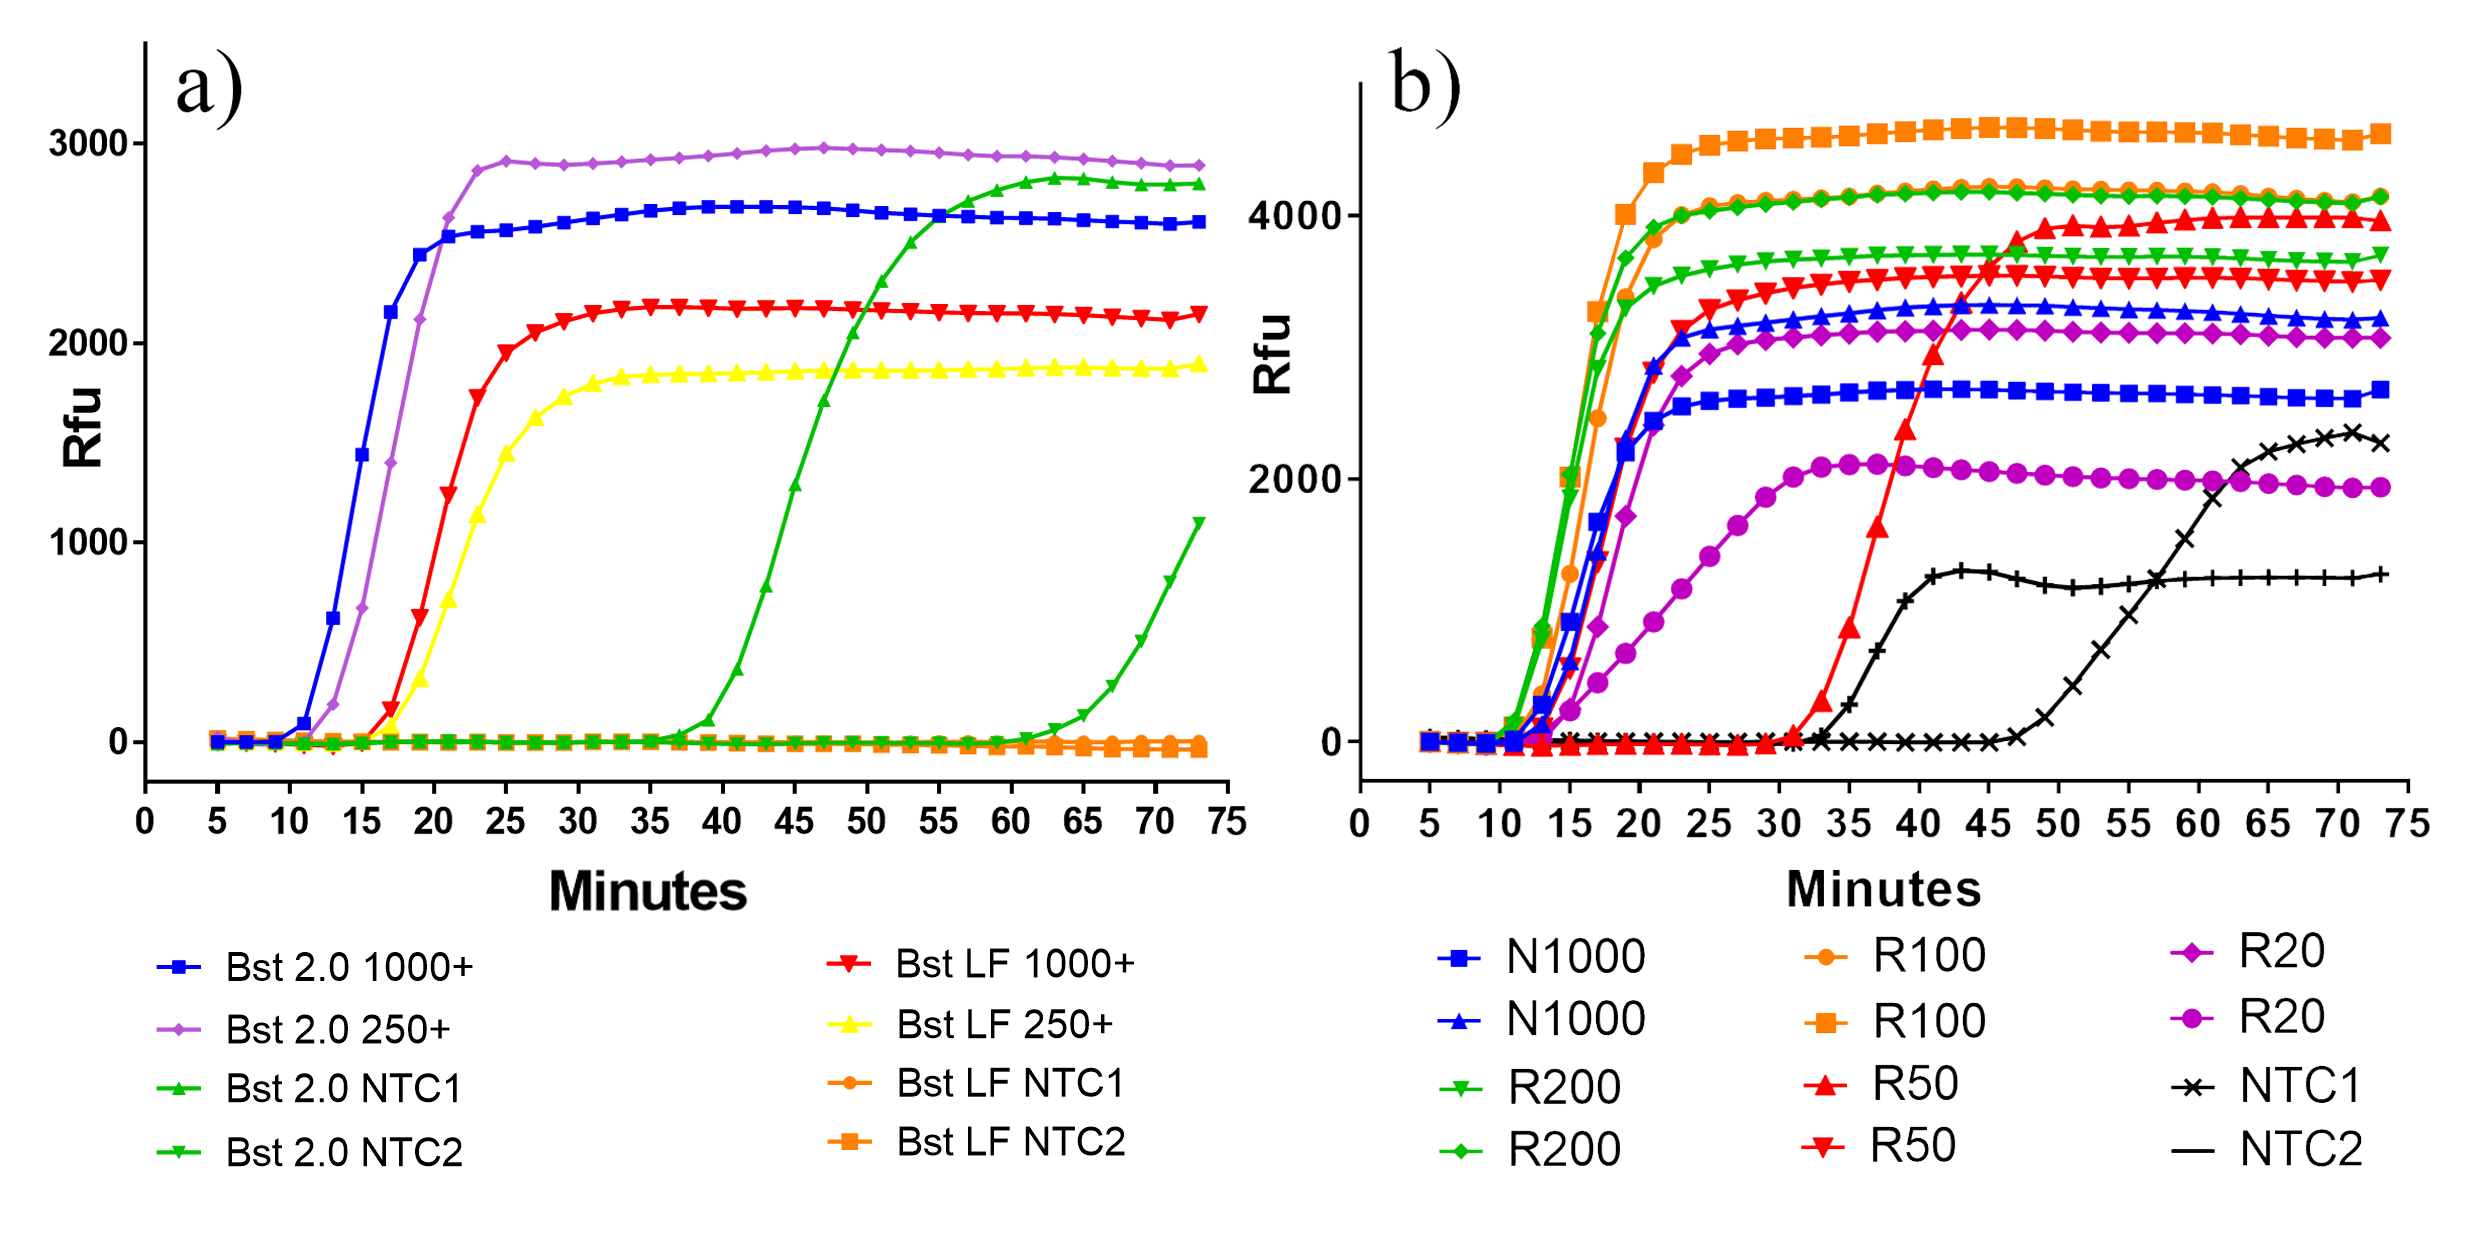
\includegraphics[width=1\textwidth]{figures/LAMP1.png}
    \caption[Real-time amplification data demonstrate rapid and sensitive detection.]{Real-time amplification data demonstrate rapid and sensitive detection. A) Bst 2.0 is more rapid than Bst LF. N250/N1000 reactions have 250/1000 copies of the N plasmid control, respectively. Incubation temperature was at 63ºC, and reaction volumes were 25 ~{\textmu}l. B) RNA controls are reverse transcribed and amplified for detection down to a single copy per microliter of the reaction. Synthetic RNA (BEI Resources) dilutions were spiked into duplicate reactions at 20, 50, 100, and 200 (R20, R50, R100, and R200) copies, in addition to non-template control (NTC) and DNA controls. These reactions used Bst 2.0 and RTx; RFU - relative fluorescence units.}
    \label{fig:LAMP1}
\end{figure}

In the first place, we compared the efficiency of two enzymes, the Bst Large-Fragment (BST-LF) and the Bst2.0 (both acquired from New England Biolabs, UK), to amplify a DNA plasmid containing the target N gene. The amplifications were carried out through Real-Time LAMP amplification following the procedure described in appendix A.1.1. The main interest in comparing these two enzymes lies in the fact that, meanwhile, the Bst2.0 is a proprietary patented enzyme, the BST-LF patent is expired, allowing anyone to replicate this system in an open source way. The results show a rapid and sensitive detection of the reactions, but even though the Bst-LF performed well, the efficiency of the Bst2.0 resulted superior (Figura 2.1(A)).

Once we decided to continue the experiments with the Bst2.0, we tested the ability for amplifying synthetic RNA controls (Bei Resources) in combination with the retrotranscriptase RTx. The specific protocol is detailed in appendix A1.2. The reactions were able to amplify the synthetic RNA in 30 minutes, with a detection limit of 20 copies per reaction (Figure 2.1(B)). However, the amplification of negative controls after 40 minutes shows the limitations of relying on just an intercalant dye to generate the signal in LAMP.

To solve this problems of the regular appearance of false positives, the set was adapted to QUASR-LAMP with the procedure described in appendix A.1.3. The resulting quencher and fluorophore probes can be found in appendix A2.2. Consequently the reactions were run with the conditions previously optimized, using as a sample different concentrations of inactivated virus (BEI Resources). The detailed protocol is described in appendix A1.5. The results of this amplification can be observed in figure 2.2(A).

These promising early results led us to present the system to the Rapid Covid testing XPRIZE, one of the most prestigious private competitions in the field of cutting-edge technologies. To test the system's robustness, the foundation sent us a blind assay comprising a 96-Well plate with unknown samples (Figure 2.2(B)). The results of this test demonstrated excellent performance and paved the way to enter the semifinals\cite{marianna_limas_xprize_2020}. Unfortunately, because we competed with more mature products, the CoronaDetective journey in the XPRIZEs faced its end after this semifinals.

These results were shared in a small pre-print at the beginning of the pandemic that was finally published recently\cite{aidelberg_corona_2021}. We aimed that other groups could use this data and protocols to develop new methods, adding our little grain of sand in the fight against SARS-CoV-2.
 
\begin{figure}[b]
    \centering
    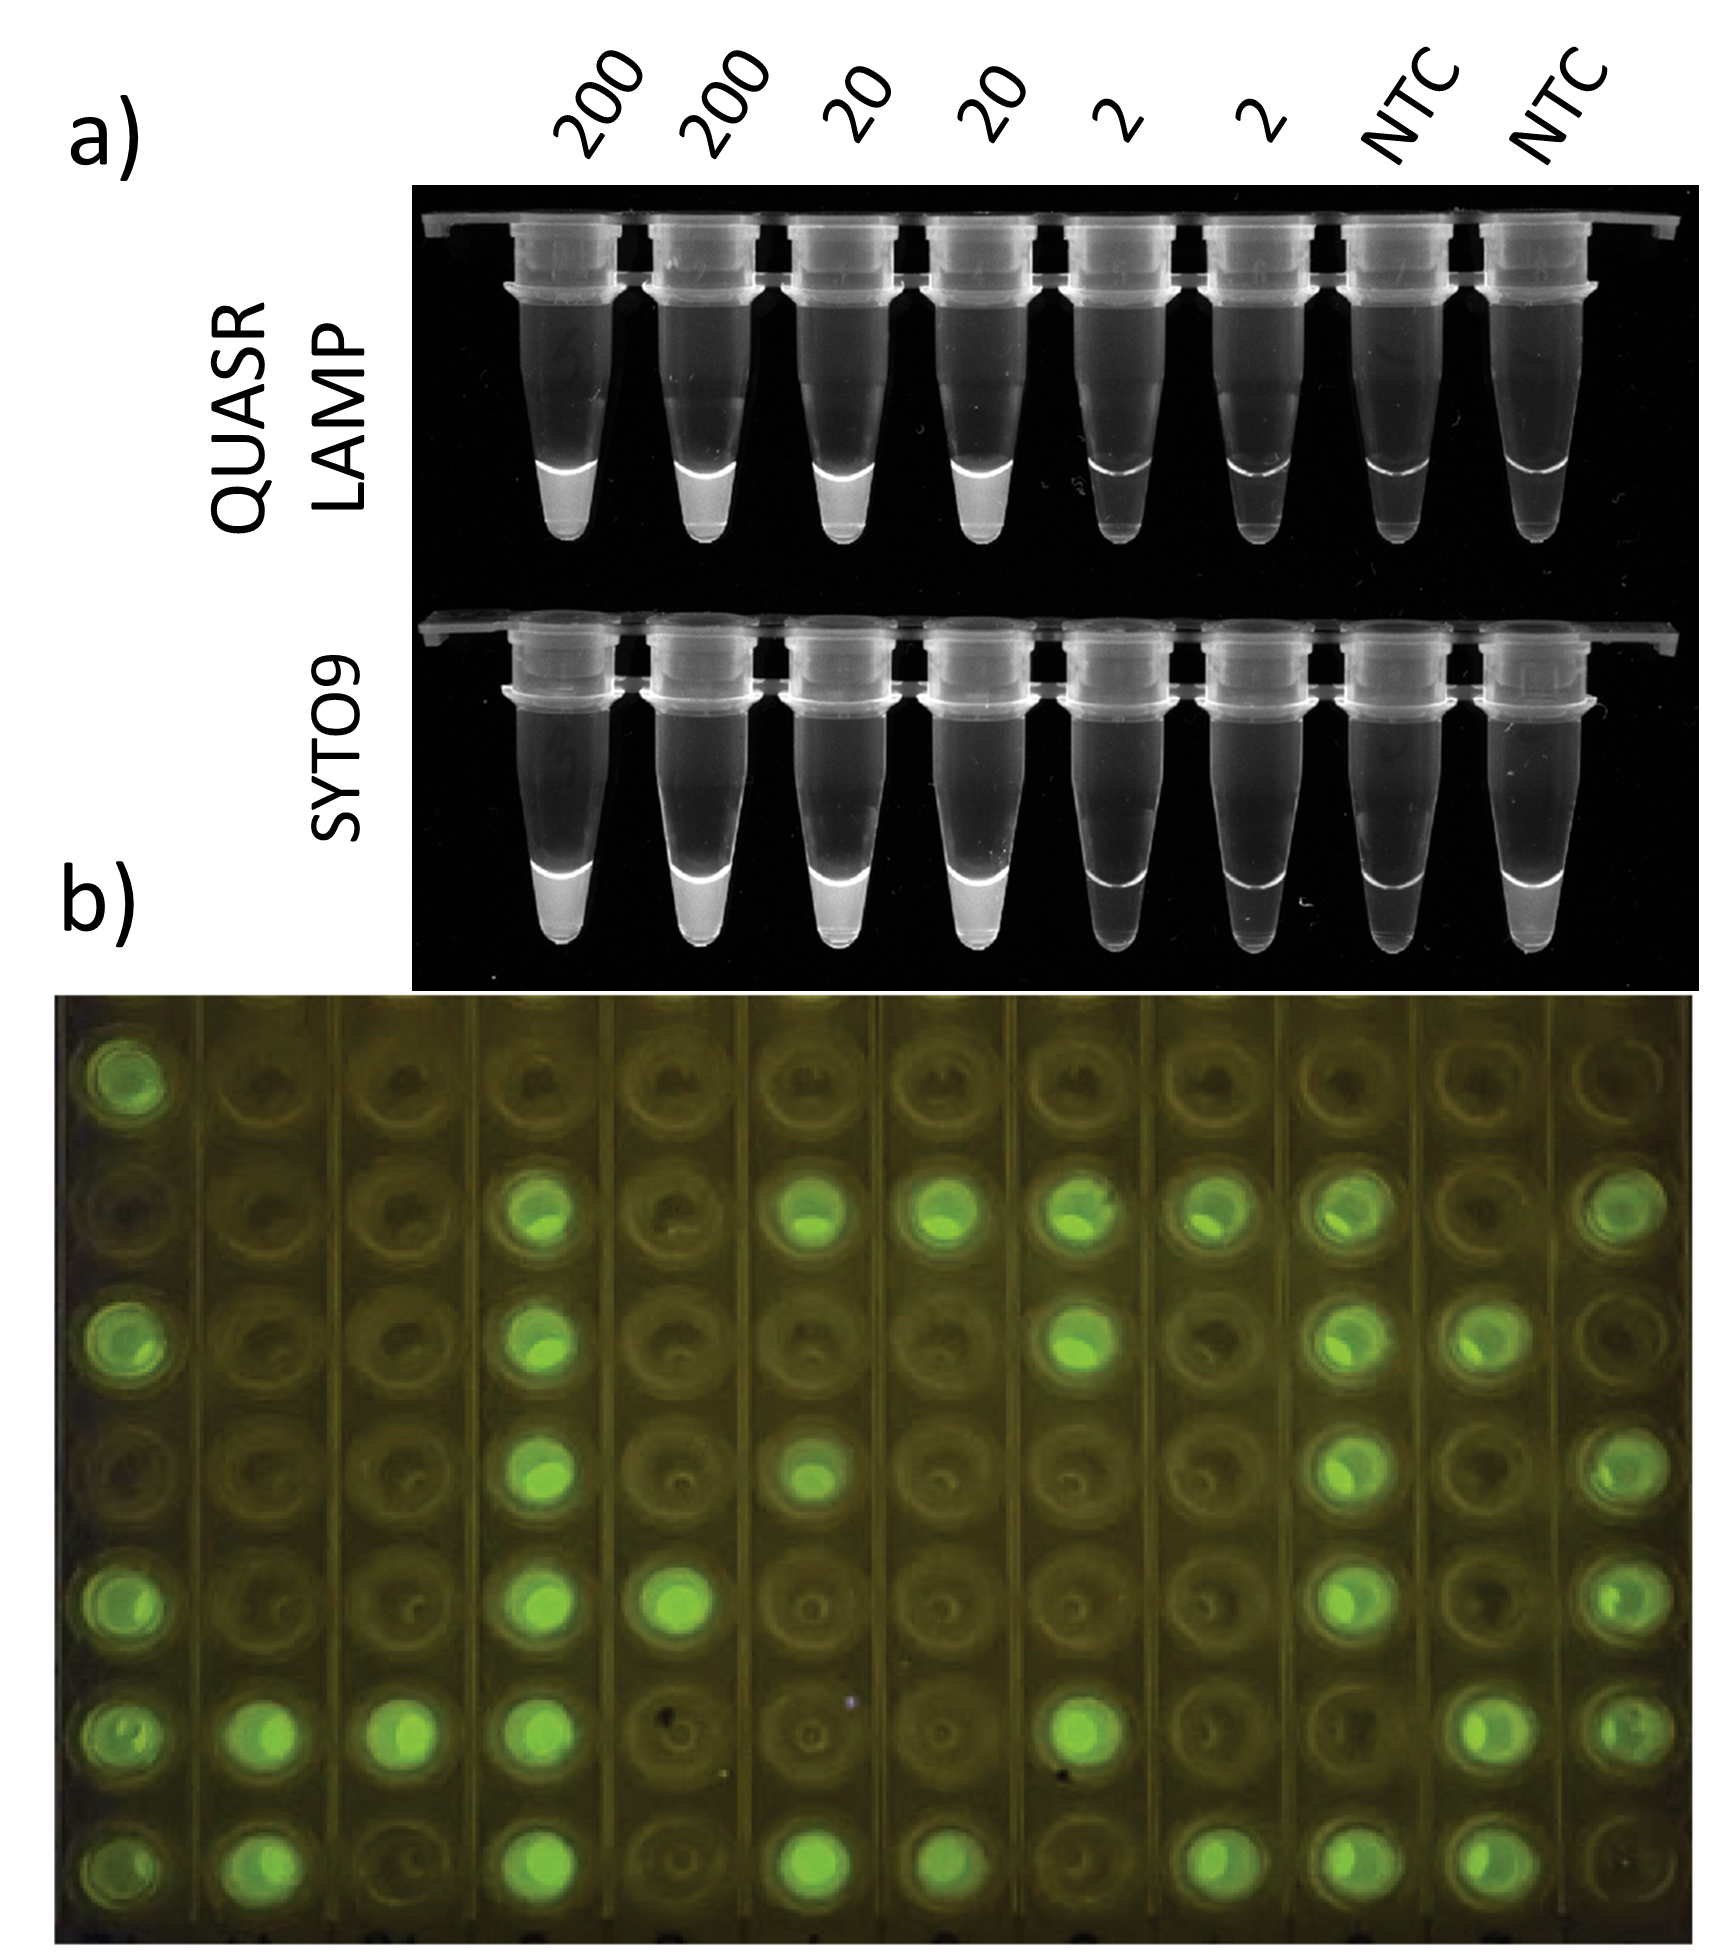
\includegraphics[width=0.59\textwidth]{figures/LAMP2.png}
    \caption[CoronaDetective qualitative results.]{ A) Results from comparison after one hour of amplification between a QUASR-LAMP and standard LAMP master mix. We used the intercalant dye SYTO9 as the signal generator as it has been described not to inhibit the amplification\cite{oscorbin_comparison_2016}. The numbers on the top indicate the total amount of inactivated viral units per reaction. Both reactions performed well, amplifying concentrations from 20 to 200 units per reaction. Both were unable to go down to 2 units per reaction. These results also demonstrate the tendency of standard LAMP to generate a signal without a template (NTC samples) contrary to the reactions already adapted to QUASR-LAMP. All the master mix, including the intercalant dye, was prepared before the incubation. The tubes have not been opened once incubated to avoid carryover contamination. All the samples were biological replicates. B) The results from the XPRIZE 96-well plate "blind test" imaged from a transilluminator.}
    \label{fig:LAMP2}
\end{figure}

\section{Liophilization of the reactions}
One of the major issues to succesfully implement diagnosis test in LMICs is the reagents sensibility to cold chain interruptions. This mainly happen becquse once the LAMP mastermix loose the refrigeration, the enzymes will start loosing activity . This requirement makes LAMP extremely difficult to implement in LMICs distant surveillance sites, especially in the tropics, where the higher temperatures represent a risk and the stable power supply is not guaranteed.

To overcome this challenge, we have designed a QUASR-LAMP master mix that perdures stable for months at room temperature. In order to achieve that, the master mix was subjected to a lyophilization process, where the solvent is removed through sublimation.Lyophilization have being broadly described to improve the room temperature shelf-life of LAMP reactions\cite{hayashida_direct_2015}\cite{garcia-bernalt_diego_progress_2019}. To ensure the reagents' stability, we included trehalose in the previously optimized master mix. Trehalose is a cryoprotection that interacts with the different reagents, immobilizing the molecules and protecting them during the lyophilization process and later. Mixtures containing a significantly high trehalose concentration change their phase from liquid to amorphous solids, in a process called vitrification, which holds trapped biological molecules retaining native structures during desiccation\cite{hayashida_direct_2015}. The liophilized master mix become significantly more resistant to temperature changes as it boost the enzymes stability.
 
 \begin{figure}[hb]
    \centering
    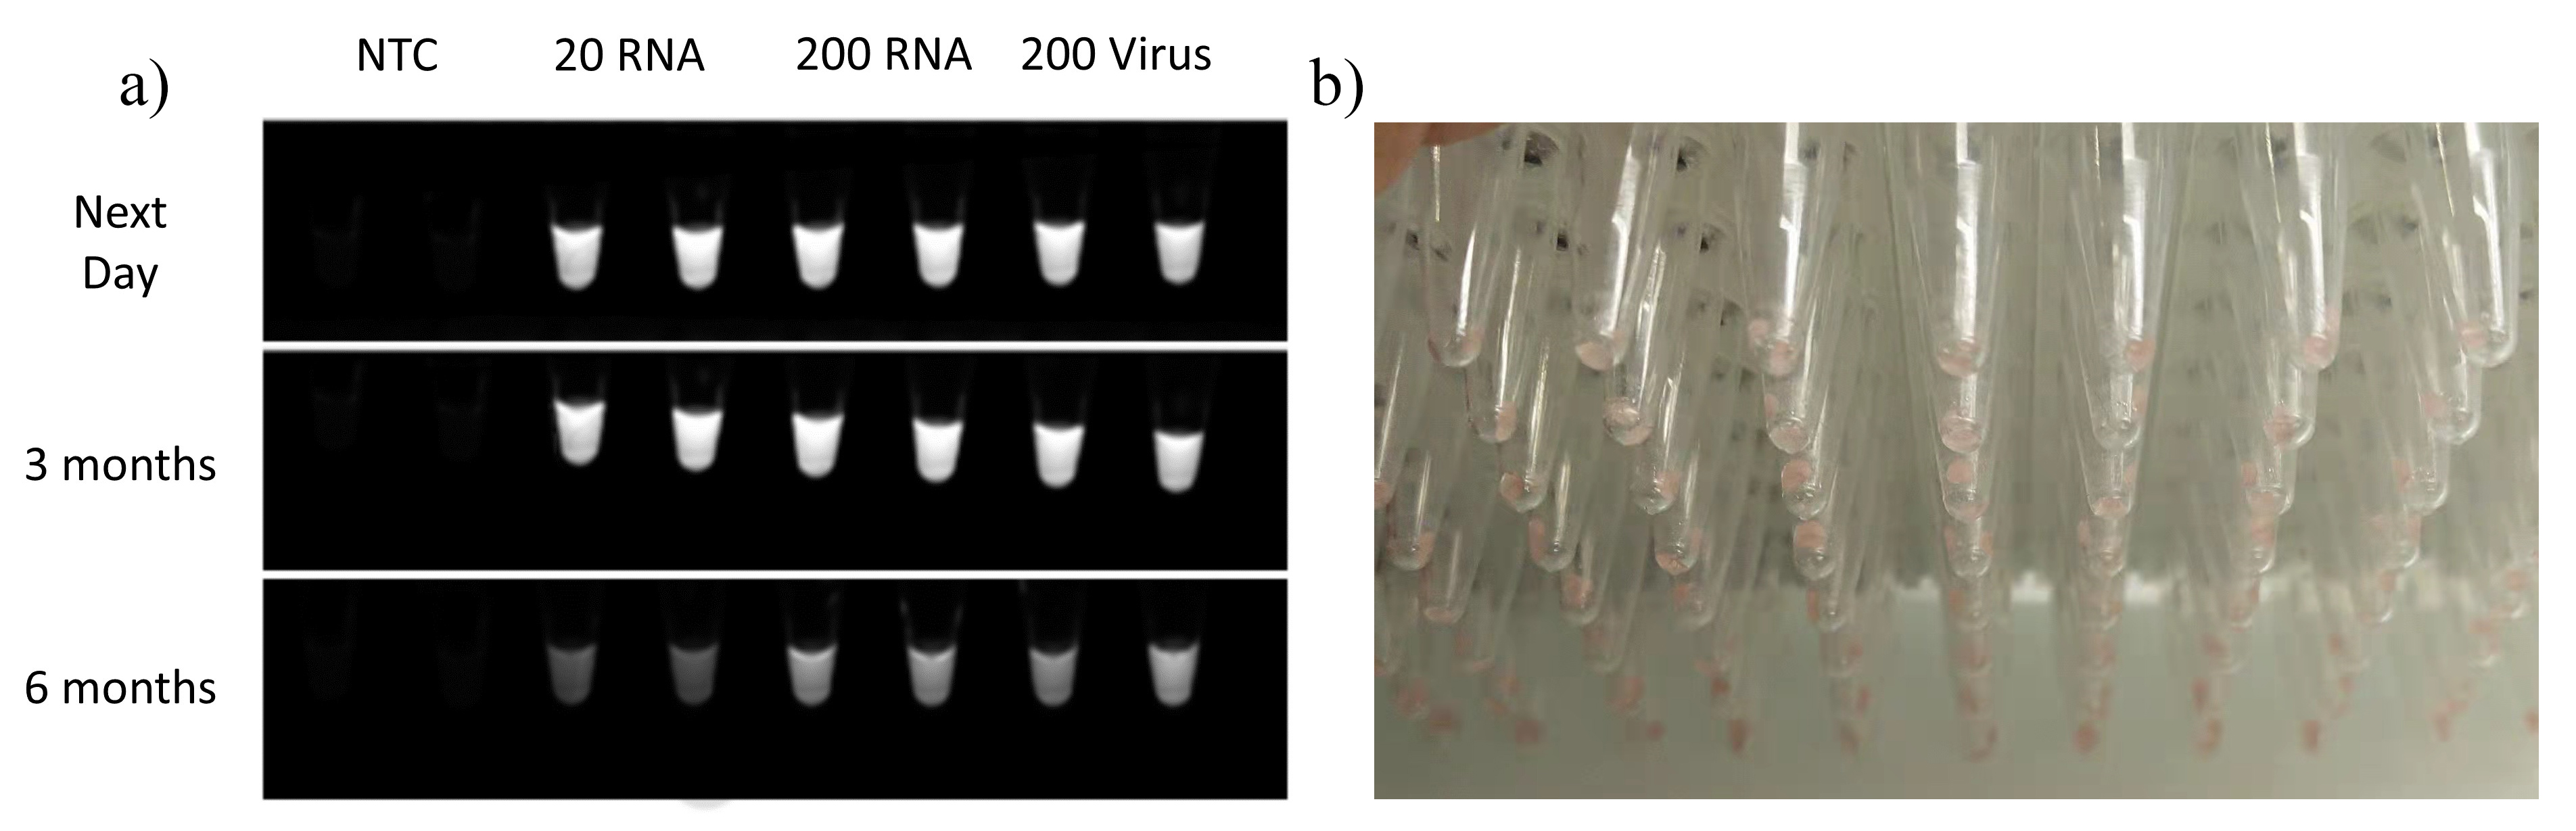
\includegraphics[width=1\textwidth]{figures/liophilization.jpg}
    \caption[CoronaDetective liophilization results.]{(A) Liophilized reactions performs well for months. However, even if they still amplify the DNA, after 6 months the speed of the reactions is significantly decreased. (B) The liophilized reactions can be observed as a pink pellet in the bottom of the tubes}
    \label{liophilization}
\end{figure}

After the lyophilization of an entire 96 well-plate, the dried master mix can be observed as a pink pellet in the bottom of the tubes (Figure 3.3(B)). The applied protocol is detailed in appendix A.1.6. 

To study the reactions stability we stored one 96 Well-Plate in a dry and dark place and we performed an amplification each 3 months until we observed a decrease in the performance (Figure 3.3(A)).

\section{Field Testing and production scalation} %cosito are you entering the computer also. Alfrede is watching you
After the promising results of section 3.1 and having improved the stability of the reactions at room temperature as described in section 3.2, we proceeded to test the reactions in the field.

For this purpose, we worked with collaborators in the low resource regions of Ghana and Chile. In Ghana, we worked with a Noguchi Institute and in Chile with the Laboratorio de Tecnologías Libres associated with the Pontificia Universidad Católica (PUC). The collaborators previously had transilluminators and a solution to incubate the reactions at 63°C for one hour, so we only sent the lyophilized reactions in the format of 96 TearAway WellPlates (Thermo Fisher Scien-
tific, Waltham, MA, USA). The reactions were carried out in clinical samples from patients with a known Ct value obtained from a previous qPCR test (Table 3.1). The most important limitations of these trials were the lack of information about the samples' pre-treatment and the freezing and thawing cycles they underwent, which probably generated the degradation of the viral RNA. 
\vspace{12pt}
% Please add the following required packages to your document preamble:
% \usepackage{multirow}
\begin{table}[]
\begin{center}
\begin{tabular}{clccccc}
\multicolumn{1}{l}{\multirow{2}{*}{}} & \multirow{2}{*}{} & \multicolumn{3}{c}{\textbf{PCR}} & \multirow{2}{*}{\textbf{Sensitivity}} & \multirow{2}{*}{\textbf{Specificity}} \\
\multicolumn{1}{l}{} &  & \textbf{Positive} & \textbf{Negative} & \textbf{Total} &  &  \\
\hline
\multirow{3}{*}{\textbf{Ghana}} & \textbf{Positive} & 32 & 0 & 32 & \multirow{3}{*}{\textbf{76.19\%}} & \multirow{3}{*}{\textbf{100\%}} \\
 & \textbf{Negative} & 10 & 53 & 63 &  &  \\
 & \textbf{Total} & 42 & 53 & \textbf{95} &  &  \\
 \hline
\multirow{3}{*}{\textbf{Chile}} & \textbf{Positive} & 53 & 0 & 53 & \multirow{3}{*}{\textbf{63.86\%}} & \multirow{3}{*}{\textbf{100\%}} \\
 & \textbf{Negative} & 30 & 41 & 71 &  &  \\
 & \textbf{Total} & 83 & 41 & \textbf{124} &  & 
\end{tabular}
\end{center}
\vspace{10pt}
\caption[CoronaDetective field testing results.]{CoronaDetective exhibited a robust specificity performance; the system perform well avoiding the generation of false positives. However, the values in the sensitivity are of concern. The sample management may partially explain the uneven results between qPCR and CoronaDetective. The qPCR was performed immediately after sample extraction and frozen for later uses. This sample management protocol can partially explain the difference in sensitivity between the Ghana and Chile trials. In Ghana, the samples were thawed for its use with CoronaDetective a couple of days later. In contrast, in Chile, they remained frozen for a week. Furthermore, in some cases the samples were even thawed and frozen before being tested, facilitating the rapid degradation of the viral RNA. These data show the need to design more robust testing protocols in the future. The raw results from the tests can be be obtained from Appendix A.2.3.}
\end{table}

Once performed the proof of concept, we studied how to produce and lyophilize the reactions on larger scales. We started comparing reagents offers from large-scale batches and exploring companies to mix, lyophilize and package hundreds of reactions. We filter these companies based on two main features; how competitive their services were and the compliance with ISO 13485, which guarantees the medical grade in the resulting products. One of the most promising results was Evik Diagnostics (Kanata, Canada), services that we are still testing at the moment. As a result of months of offers and comparisons, Table 3.2 shows the cost to produce a CoronaDetective reaction.
\begin{table}[]
\begin{center}
\begin{tabular}{lr|lr}
\textbf{Component} & \multicolumn{1}{l|}{\textbf{Reaction price (USD)}} & \textbf{Component} & \multicolumn{1}{l}{\textbf{Reaction price (USD)}} \\ \hline
RTx retrotranscriptase & 0.91 & Caps & 0.05 \\
Mixing \& lyophilization  & 0.55 & Primer Mix & 0.04 \\
Bst polymerase & 0.22 & Tubes & 0.04 \\
dNTPs & 0.17 & \textbf{Total} & 1.99
\end{tabular}
\end{center}
\vspace{10pt}
\caption{Summary of production costs per CoronaDetective reaction.}
\end{table}


\section{Conclusion}
This chapter describes the successful design of a simple, inexpensive, robust and room-temperature stable SARS-CoV-2 diagnostic test that meets all the requirements for its implementation in developing countries. In addition, as described in the final part of the previous section, large-scale production studies have been carried out, with an estimated price of around \$2 per reaction that will decrease significantly depending on the production size. Furthermore, as the reaction is based on one enzyme, the system is simple enough to open the door for local production and manufacturing. The most important limitation of our trials were the lack of quality clinical samples to accurately benchmark the system against the current diagnosis gold-standard, the qPCR.

Another great advantage of this method is that it can be easily scalable from SARS-CoV-2 detection to other relevant diseases, just by changing the primers and performing an easy optimization. We have demonstrated it adapting the system to other targets, such as the GMO detective (For detecting common transgenic elements in the food industry)\cite{guy_aidelberg_gmo_2018} or detecting fungal infections by \emph{Phytophthora cinnamomi} in chestnuts trees (Work in preparation). However, during the implementation in the field, it became evident that we relied on laboratories that already had previously established laboratories with a basic level of equipment to incubate and analyze the reactions. This centralizes the diagnosis to a handful of laboratories in the LMICs capitals, keeping healthcare bottlenecks and moving away from the vision of a decentralized diagnosis throughout the region.

In the following chapter we will describe two protable open-source devices, designed during this thesis, that will not only enable the incubation and qualitative QUASR-LAMP analysis, but will open the door to the quantitative analysis that was previously limited to laboratories with very expensive (~40000USD) real-time PCR machines. The democratization of these technologies will allow remote regions to expand their capabilities achieving a better diagnosis and performing their own primer design and reaction optimization.


